\documentclass[a4paper, 12pt]{article}
\usepackage[utf8]{inputenc}
\usepackage[T1]{fontenc}
\usepackage[french]{babel}
\usepackage{graphicx}
\usepackage{amsmath}
\usepackage{amssymb}
\usepackage{graphicx}
\usepackage{float}
\usepackage{hyperref}
\usepackage{geometry}

\geometry{hmargin=1.5cm,vmargin=4cm}
\pagestyle{headings}

\title{Rapport final de Développement Web 2}
\author{Lucas Jouvet, Francis Kempenaers et Tao Grolleau}
\date{\today}

\begin{document}

\maketitle

\begin{abstract}
  Nous détaillons dans ce rapport les principales fonctionnalités de notre application. Le chef de projet désigné est Tao Grolleau.
\end{abstract}

\newpage

\section{Description de l'application}

Les documents traités sont des fichiers de code source, pouvant être modifiés par des utilisateurs qui peuvent former des groupes. Les documents peuvent être soit publics, soit privés. 

Dans le cas des documents privés, seuls les utilisateurs auxquels le propriétaire à donné l'accès peuvent modifier le document, toute modification est définitive. 

N'importe quel utilisateur peut voir les documents publics et proposer une modification. Seul le propriétaire du document est en mesure d'accepter ces modifications ou de les supprimer. Les modifications peuvent être vues par n'importe quel utilisateur.

Un utilsateur sans compte peut créer une page d'édition temporaire, et il peut partager le lien. Le document peut être exporté en un fichier local. Le document est détruit lorque le créateur quitte la page.

\subsection{Principales fonctionnalités}

La communication se fait par chat, et celui-ci n'est présent que sur les pages d'édition où l'on peut modifier les documents. Chaque utilisateur a une messagerie, et tous les autres utilisateurs peuvent lui laisser un message.

Chaque utilisateur a la possibilité de créer un groupe, il en devient alors l'administrateur. Il peut ainsi inviter de nouvelles personnes ou en supprimer du groupe. Chaque groupe a une page unique, qui contiendra le nom des membres, les logs de modification (sans possiblité de revenir en arrière), et les noms des différents fichiers.

Chaque fichier a des commentaires qui lui sont associés, ceux-ci ne peuvent être supprimés.

\subsection{Différents diagrammes}
\begin{figure}[H]
  \begin{center}
    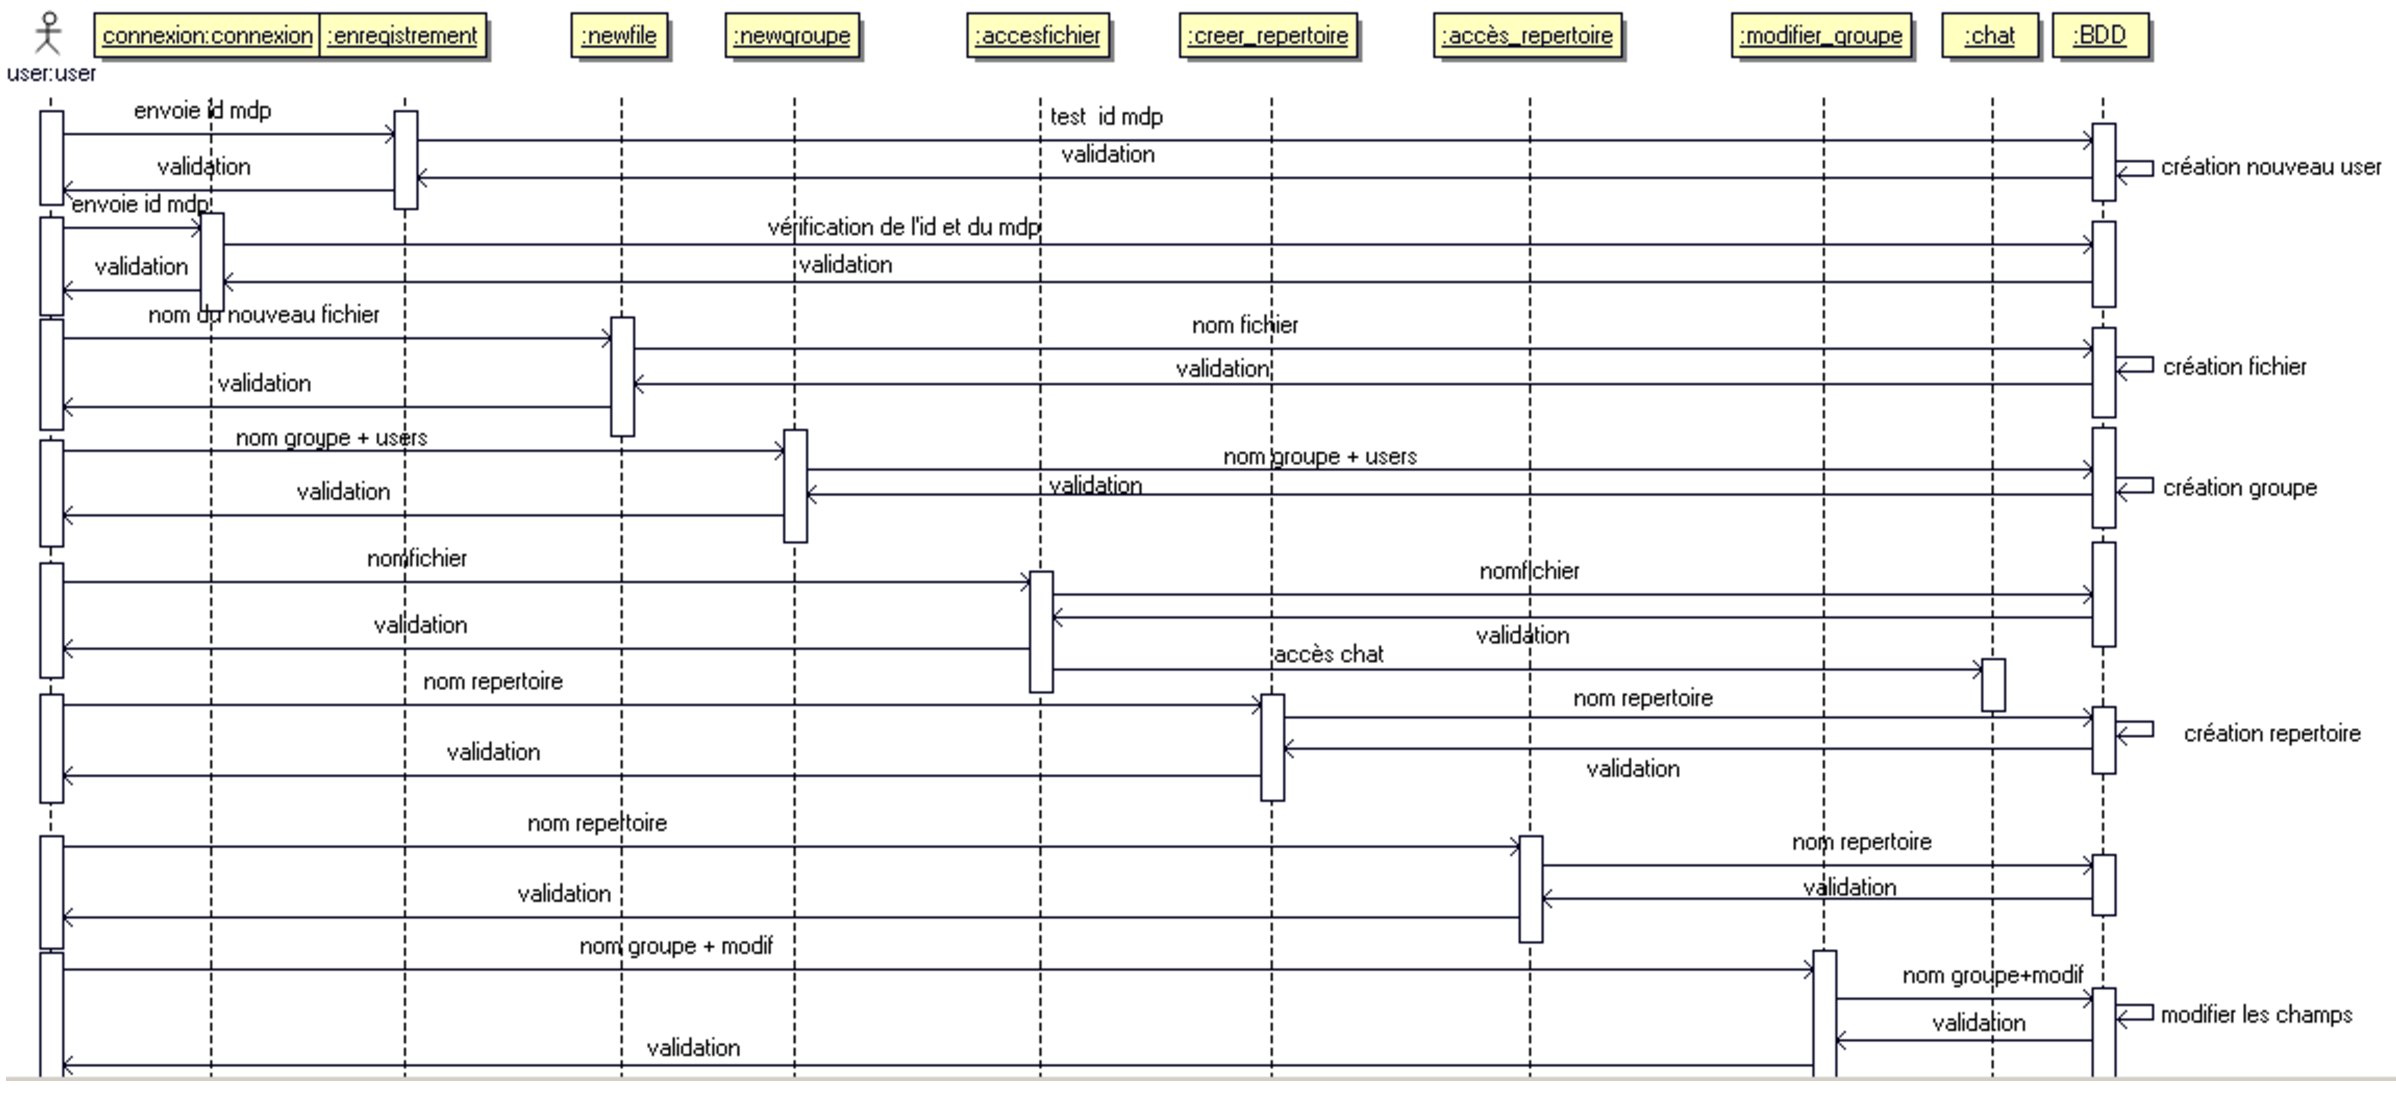
\includegraphics[scale=0.4]{sequence.pdf}
  \end{center}
  \caption{Diagramme de séquence}
\end{figure}
\begin{figure}[H]
  \begin{center}
    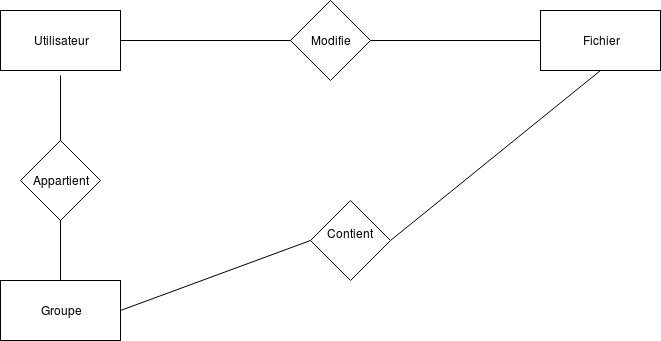
\includegraphics[scale=0.7]{EntiteAssociationBDD.png}
  \end{center}
  \caption{Diagramme entitée association}
\end{figure}
\begin{figure}[H]
  \begin{center}
    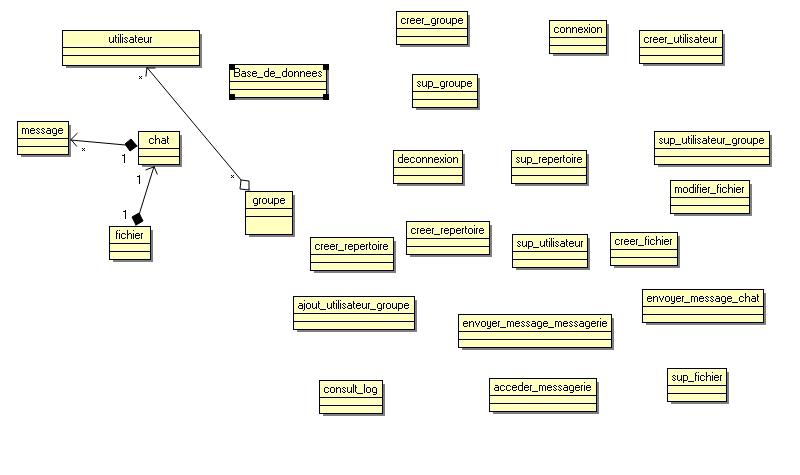
\includegraphics[scale=0.7]{Diagramme_classe.png}
  \end{center}
  \caption{Diagramme de classes}
\end{figure}

\begin{figure}[H]
  \begin{center}
    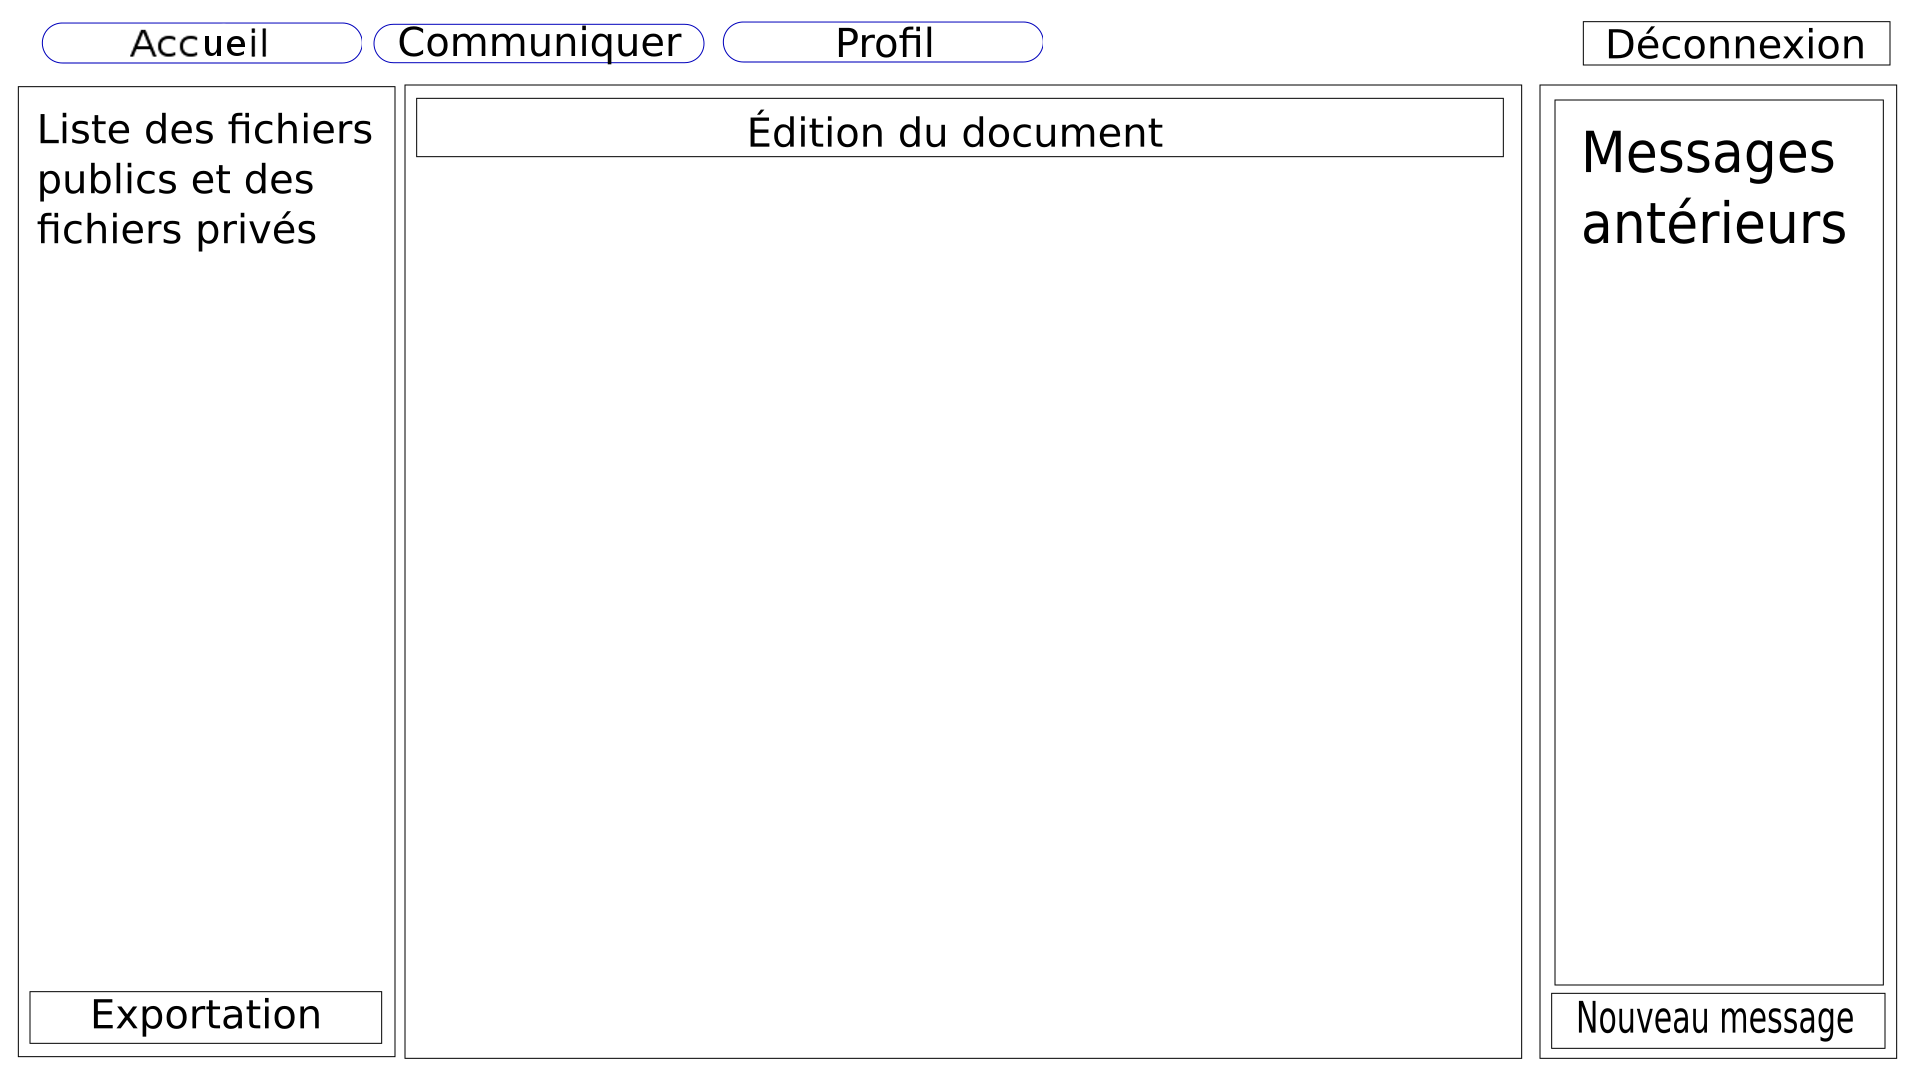
\includegraphics[scale=0.3]{edition.png}
  \end{center}
  \caption{Page d'édition}
\end{figure}

\begin{figure}[H]
  \begin{center}
    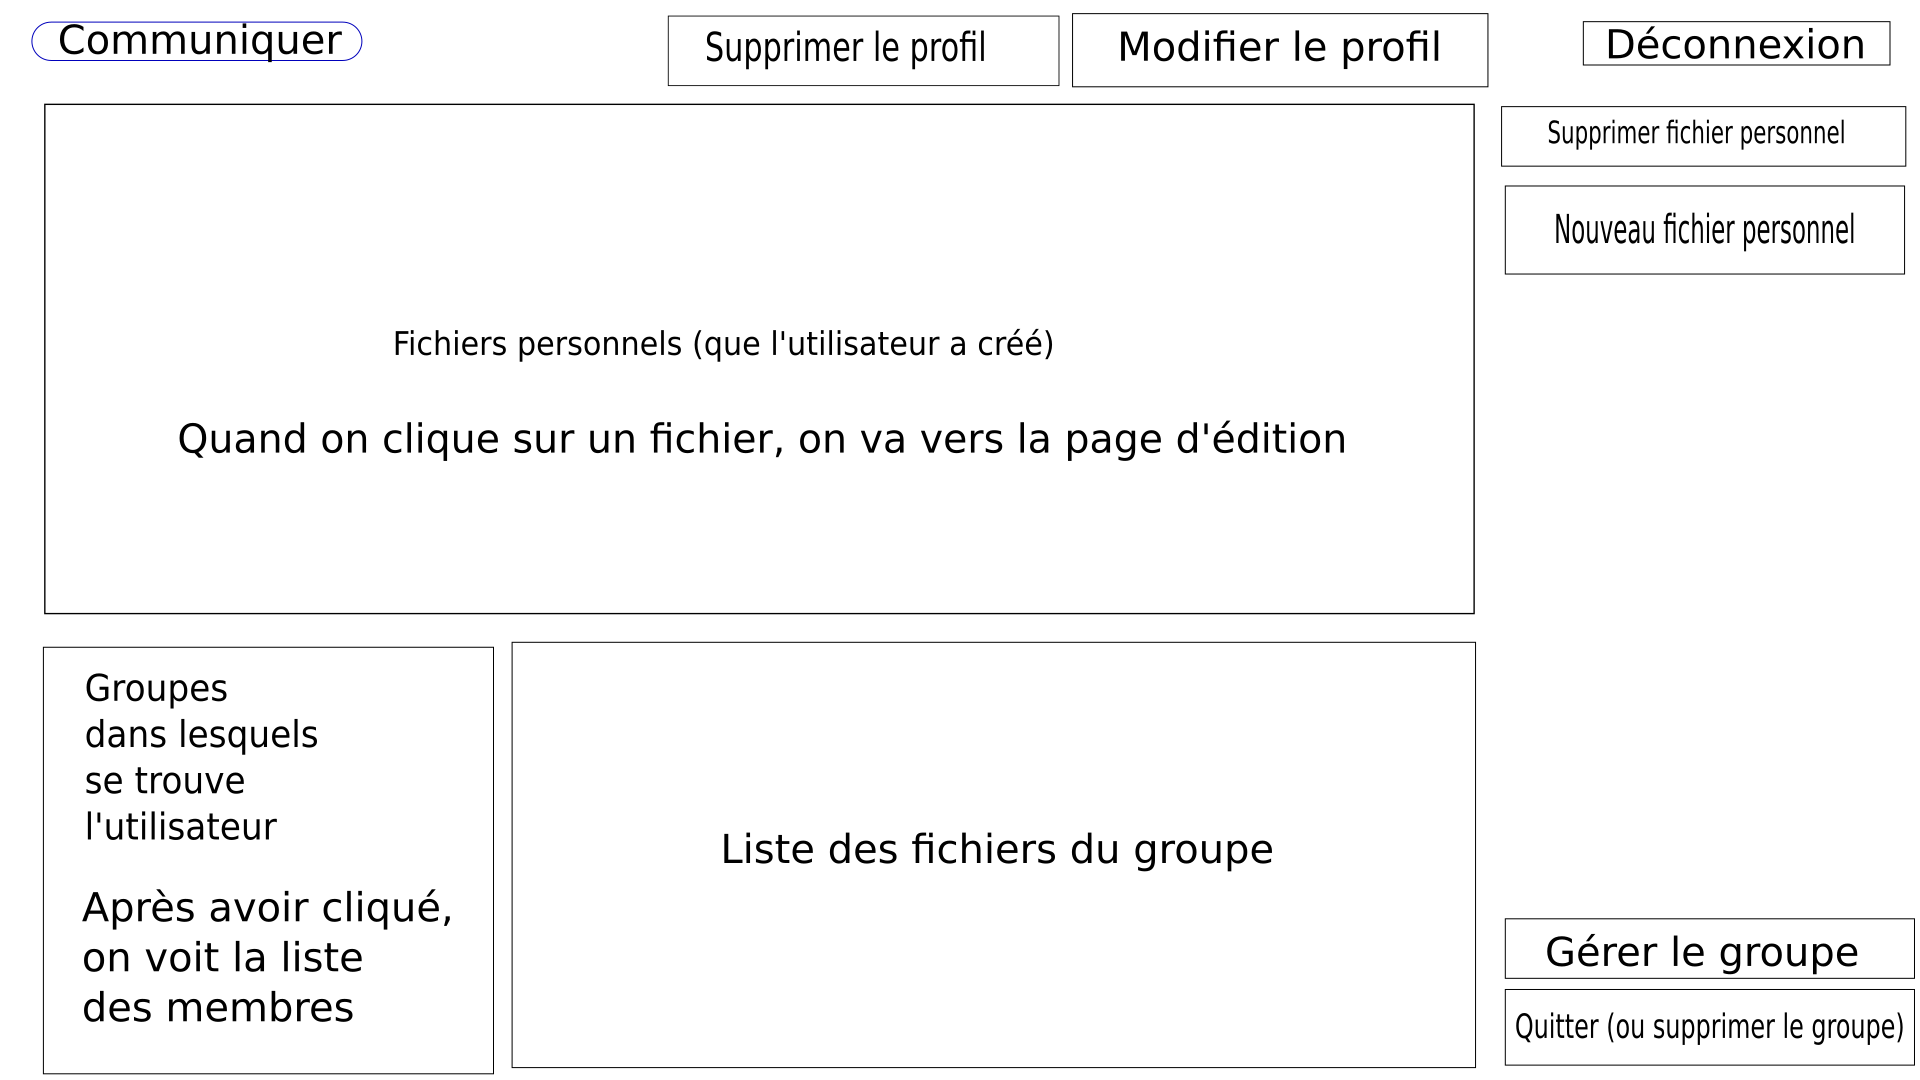
\includegraphics[scale=0.3]{profil.png}
  \end{center}
  \caption{Page du profil}
\end{figure}

\begin{figure}[H]
  \begin{center}
    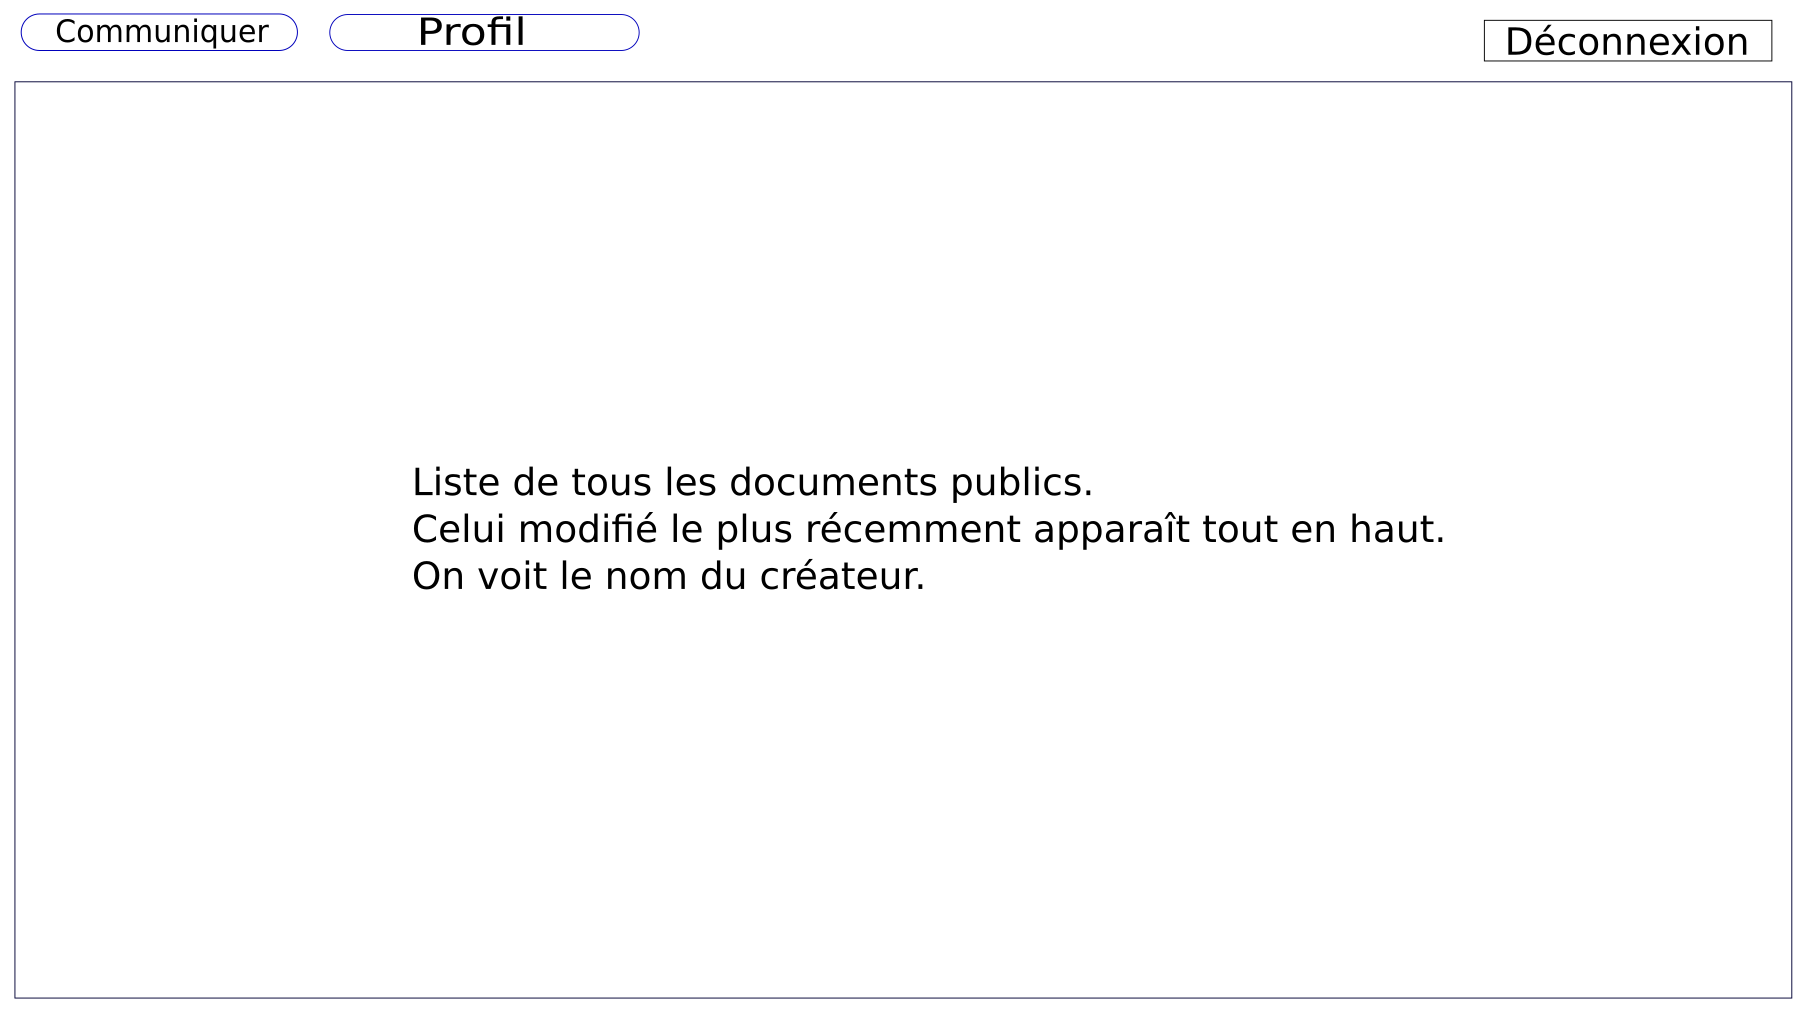
\includegraphics[scale=0.3]{acceuil.png}
  \end{center}
  \caption{Page d'accueil}
\end{figure}

\begin{figure}[H]
  \begin{center}
    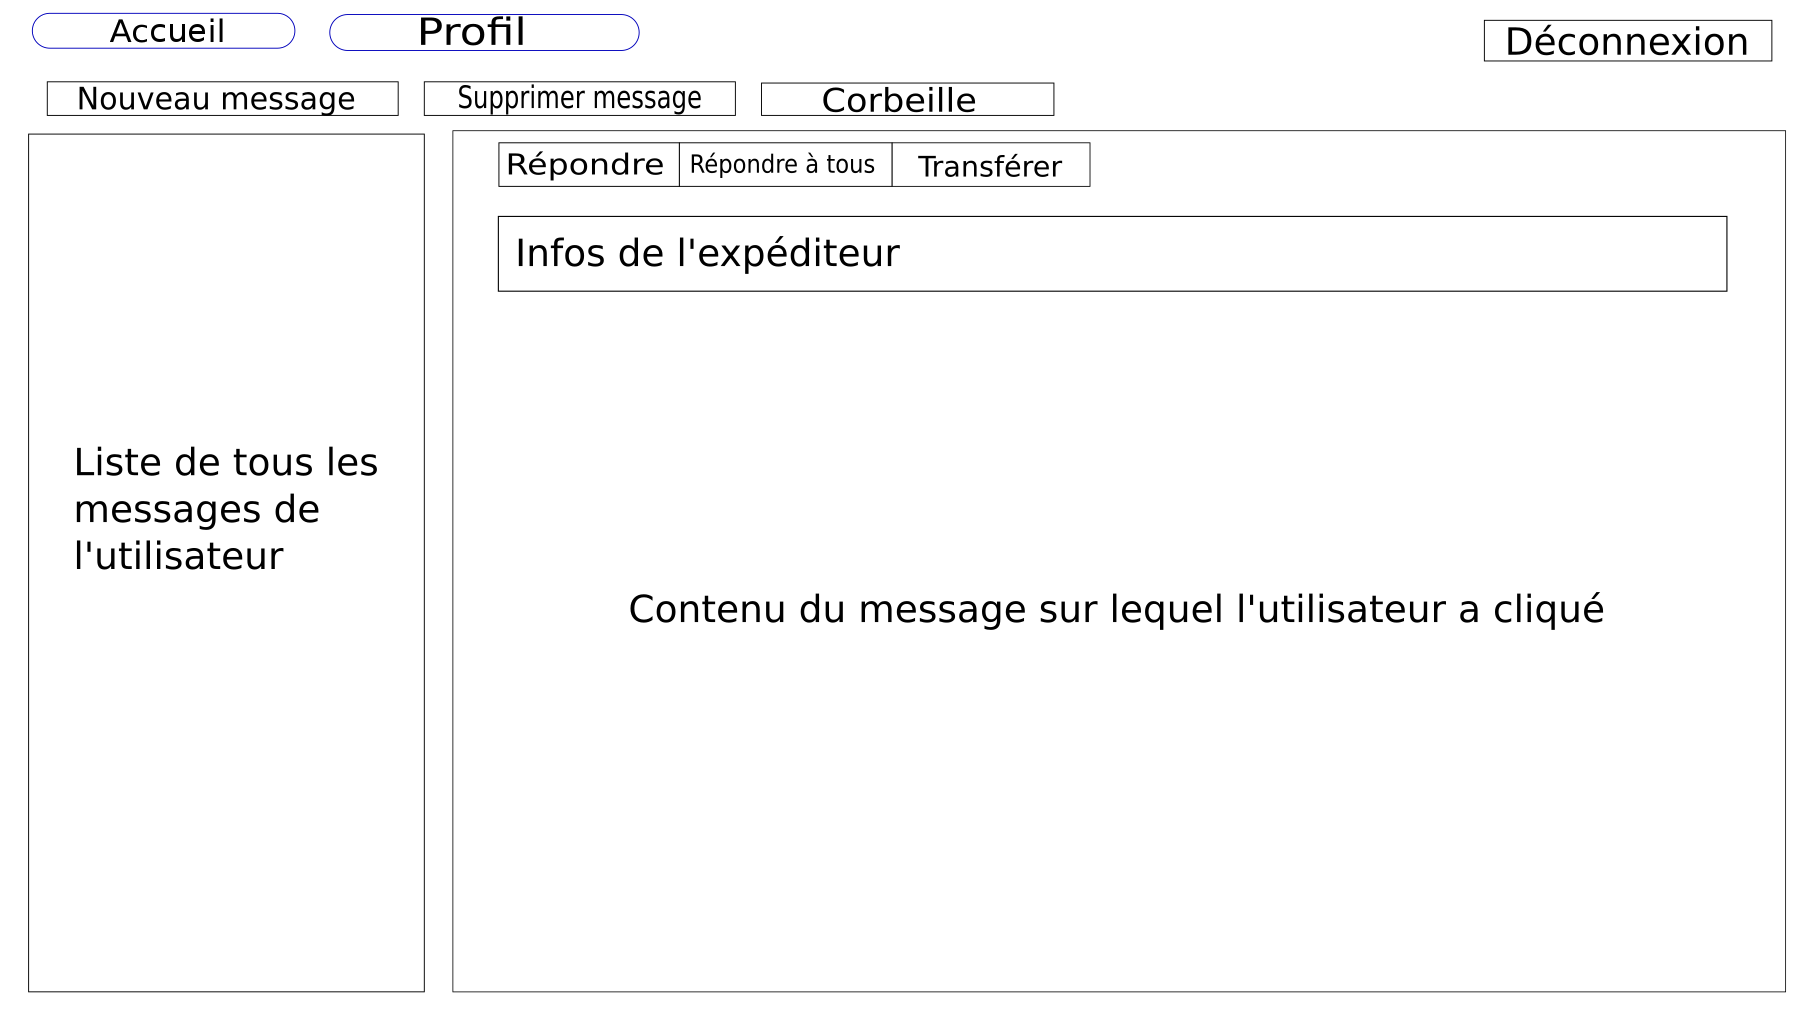
\includegraphics[scale=0.3]{communiquer.png}
  \end{center}
  \caption{Page de messagerie}
\end{figure}

\section{Technologies utilisées}

Nous allons utiliser Swing pour le client lourd, des jsp et servlets pour le client léger. Conformément à l'architecture MVC : Les servlets seront utilisés pour traiter les requêtes, et les jsp pour y répondre. Pour le xml nous pensons peut-être l'utiliser pour importer et exporter des groupes d'utilisateurs.

\section{Rôles des membres du groupe}

Cela sera sûrement détaillé plus tard, et sujet à changement.
Mais pour commencer, Lucas Jouvet va s'occuper du client léger, Francis Kempenaers va s'occuper du client lourd et Tao Grolleau va s'occuper de la base de données et de son implémentation dans les deux clients.

\end{document}
